\documentclass[a4paper,11pt]{article}
\usepackage[utf8]{inputenc}
\usepackage{minted}
\usepackage{amsmath}
\usepackage{float}
\usepackage{footmisc}
\usepackage{graphicx}
\usepackage{multirow}
\usepackage[toc,page]{appendix}

\graphicspath{{./figures/}}

\title{\textbf{12. Graphs}}
\author{Kristiāns Vinters}
\date{Fall 2023}

\begin{document}
    \maketitle
    \section*{Introduction}

    I solved the assignment in Go. I used Go because I want to become more familiar with it. Source code and benchmark data is available on GitHub\footnote{https://github.com/Phanty133/id1021/tree/master/12-graphs}.

    \section*{Implementation}

    I wrote all graph-related code in the package \texttt{trains}. I had three structs - \texttt{City}, \texttt{Connection}, and \texttt{NetworkGraph} that provides an interface for the graph.

    \begin{minted}{go}
type City struct {
    Name      string
    Neighbors []Connection
}

type Connection struct {
    City *City
    Dist int // In minutes
}

type NetworkGraph struct {
    cities    [][]*City
    NumCities int // Used for preallocating visited cities array
}
    \end{minted}

    \texttt{NetworkGraph.AddCity()} and \texttt{NetworkGraph.LookupCity()} functions are implemented the same as in the previous HashMap assignment with the hashing function given for this assignment.

    To initialize the graph, I created the function \texttt{NetworkGraph.FillData()} that takes in the columns of the data CSV file.

    \begin{minted}{go}
func (n *NetworkGraph) FillData(from []string, to []string, dist []int) {
    for i := 0; i < len(from); i++ {
        // Check if the city nodes already exist,
        // if not, create them
        fromCity := n.LookupCity(from[i])
        toCity := n.LookupCity(to[i])

        if fromCity == nil {
            fromCity = &City{from[i], nil}
            n.AddCity(fromCity)
        }

        if toCity == nil {
            toCity = &City{to[i], nil}
            n.AddCity(toCity)
        }

        // Skip duplicate connections just in case
        if fromCity.IsConnected(toCity) {
            continue
        }

        fromCity.Connect(toCity, dist[i])
        toCity.Connect(fromCity, dist[i])
    }
}
    \end{minted}

    I implemented all of the depth-first pathfinding functions with recursion. The \texttt{NetworkGraph} struct had initializer methods \texttt{DepthFirstDistance}, \texttt{DepthFirstDistanceNoLoop}, \texttt{DepthFirstDistanceNoLoopMaxed}, which took in \texttt{from} and \texttt{to} string arguments and called the corresponding recursive methods on the \texttt{City} struct, looked up with the \texttt{from} arg.

    All of the methods are implemented similarly. I'll use the NoLoopMaxed method as an example, as it incorporates logic from both other functions.

    \begin{minted}{go}
func (n *NetworkGraph) DepthFirstDistanceNoLoopMaxed(
    from string,
    to string
) (int, error) {
    // Find both cities and find if they're valid
    fromCity := n.LookupCity(from)
    toCity := n.LookupCity(to)

    if fromCity == nil || toCity == nil {
        return 0, errors.New("city not found")
    }

    // Initialize the visited path array
    visited := make([]string, n.NumCities)

    return fromCity.shortestDistanceNoLoopMaxed(toCity, visited, -1, -1)
}

func (c *City) shortestDistanceNoLoopMaxed(
    to *City,
    visited []string,
    closestDistFound int, // -1 initially, then the closest distance found
    distLeft int, // -1 initially, then the distance left in the current path
) (int, error) {
    if c == to {
        return 0, nil
    }

    // If a closest dist is found, check for remaining distance.
    // I have two arguments for both, as it seemed more robust to
    // have one that is mainly used as a flag that a closest distance
    // is found, and the other for tracking the remaining distance.
    if closestDistFound != -1 && distLeft <= 0 {
        return 0, errors.New("max distance exceeded")
    }

    minDist := -1

    for _, con := range c.Neighbors {
        // Skip if path already contains city
        if contains(visited, con.City.Name) {
            continue
        }

        // Recursively call the function on the neighbor
        dist, err := con.City.shortestDistanceNoLoopMaxed(
            to,
            append(visited, c.Name),
            closestDistFound,
            distLeft-con.Dist,
        )

        if err != nil {
            continue
        }

        // If the distance through the neighbor is found,
        // check if it's the shortest distance found so far
        if minDist == -1 || dist+con.Dist < minDist {
            minDist = dist + con.Dist

            if closestDistFound == -1 || minDist < closestDistFound {
                closestDistFound = minDist
                distLeft = closestDistFound
            }
        }
    }

    if minDist == -1 {
        return 0, errors.New("no path found")
    }

    return minDist, nil
}
    \end{minted}

    \section*{Benchmarks}
    \subsection*{Hashmap collisions}

    The given hash function had 3 buckets with collisions. The cities \texttt{Gävle}, \texttt{Kiruna}, \texttt{Luleå} had a hash of $334$, \texttt{Katrineholm} and \texttt{Värnamo} hashed to $335$, and \texttt{Emmaboda} and \texttt{Uddevalla} hashed to $155$.

    \subsection*{Pathfinding implementations}

    I benchmarked the three pathfinding implementations with the city pairs given in the assignment. For the naive implementation, I started with a max distance of $300$ and if the path wasn't found, I increased it $\times1.5$.

    \begin{figure}[H]
        \centering
        
        \hspace*{-45pt}\begin{tabular}{c|c|c|c|c|c}
            \textbf{From} & \textbf{To} & \textbf{Dist, min} & \textbf{Naive, ms} & \textbf{NoLoop, ms} & \textbf{NoLoopMaxed, ms} \\
            \hline
            \hline
            Göteborg & Stockholm & 211 & 7 & 475 & 0.06 \\
            Göteborg & Umeå & 705 & N/A & 1150 & 62 \\
            Göteborg & Sundsvall & 515 & N/A & 900 & 44 \\
            Malmö & Göteborg & 153 & 9 & 930 & 0.09 \\
            Malmö & Stockholm & 273 & 8 & 910 & 0.05 \\
            Malmö & Kiruna & 1162 & N/A & 2950 & 277 \\
            Stockholm & Sundsvall & 327 & 1050 & 700 & 6.4 \\
            Stockholm & Umeå & 517 & N/A & 980 & 13 \\
            Sundsvall & Umeå & 190 & 0.02 & 1970 & 730 \\
            Umeå & Göteborg & 705 & 32000 & 880 & 0.19 \\
        \end{tabular}
        \caption{Pathfinding results}
        \label{fig:pathfinding}
    \end{figure}

    The naive implementation didn't finish for all routes, whereas both others did. Interestingly, the times on average for the routes that did finish were faster for the naive implementation than for the simple NoLoop implementation. This is probably because the NoLoop implementation needs to do a linear search over the path for every recursive function call. The NoLoopMaxed implementation was the fastest for all routes because it didn't loop and minimized the number of recursive calls.

    \subsection*{Distances from Malmö}

    I ran an additional benchmark to measure the time it takes to find the shortest distance from Malmö to all other cities. I used the NoLoopMaxed implementation for this. All searches are repeated 50 times and the median time taken. All measured times are exported to a CSV file then plotted in LibreOffice Calc (fig. \ref{fig:path-times}). As expected, the time taken increases with the distance, however it's non-linear.

    \begin{figure}[H]
        \centering
        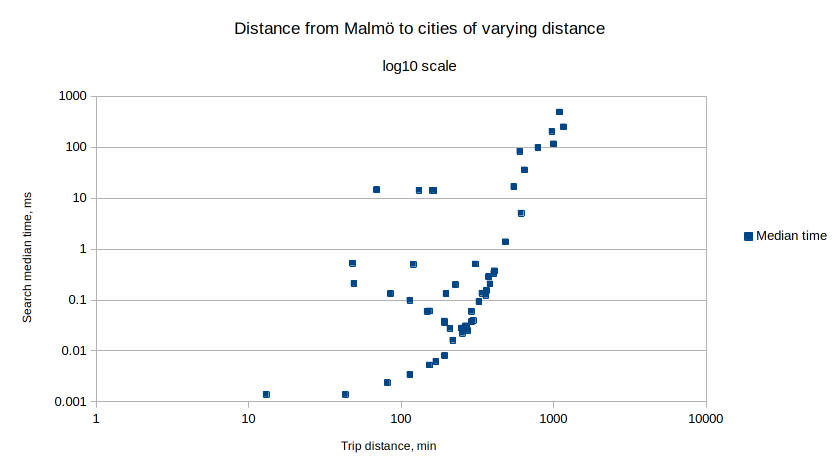
\includegraphics[width=\textwidth]{dists.png}
        \caption{Median lookup time vs route time}
        \label{fig:path-times}
    \end{figure}

    \begin{figure}[H]
        \centering
        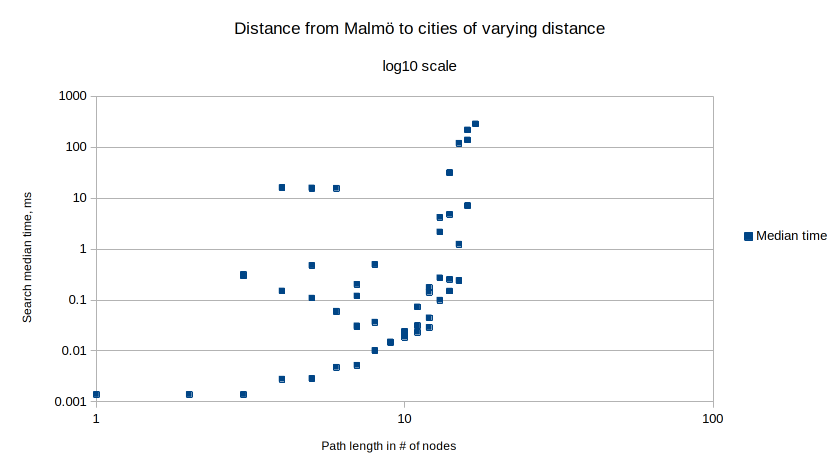
\includegraphics[width=\textwidth]{dists-paths.png}
        \caption{Median lookup time vs route distance in \# of nodes}
        \label{fig:path-nodes}
    \end{figure}
\end{document}
